\subsection{Prakses gaita}
\subsubsection{Uzdevumu dalīšana}
Izpilddirektors vai izpilddirektora vietnieks sazinās ar potenciālajiem un esošajiem klientiem un saņem informāciju par jaunu projektu izstrādi vai jau esoša projekta elementu atjaunināšanu vai uzlabošanu. Prakses autore saņem informāciju par klientu vēlmēm un uzsāk uzdevuma izpildi.
\par Pie jauna projekta izstrādes pēc klienta vēlmēm tiek veikta ienākošo failu datu kartēšana, izstrādātas datu vizuālās veidnes, atbilstošie skripti datu apstrādei un datu maršrutēšanai, testi, tiek veikta vizuālās testēšanas vietnes konfigurēšana un koda pārbaude un gatavošana gala lietotāja izmantošanai, veidojot zaru saplūšanas pieprasījumu (angl. merge request) \texttt{Gitlab} platformā. Izstrādes laikā pēc nepieciešamības no klienta tiek iegūta papildinformācija par esošajiem datiem un to apstrādi. Pēc koda izstrādes klients veic projekta testēšanu, izsakot papildus vēlmes vai labojumus. Pēc klienta apstiprinājuma projekts tiek pielaists izmantošanai produkcijā.
\par Projekta elementu atjaunināšana notiek līdzīgi jauna projekta izstrādei - tiek noskaidrotas klienta vēlmes, izstrādāti papildinājumi vai atjauninājumi, notiek koda testēšana. Pēc veiksmīgas koda izstrādes un klienta apstiprinājuma produkcijā esošais kods tiek atjaunots.

\subsubsection{Izstrādātie darbi}
Divu mēnešu laikā atskaites autore turpināja izstrādi uzsāktajam projektam datu kartēšanu trijiem datu formātiem, to testēšanu un validēšanu. Tika atjaunināti jau produkcijā esošo kodi ar izteiktajām klienta vēlmēm. Tikai izstrādāta jauna e-pasta veidne un testēta failu maršrutēšanas kvīts loģika.

\subsubsection{dhl}
\par Prakses laikā tika pastāvīgi atjaunota jau iesākta datu kartēšana jaunam kompānijas klientam. Formātam jāatbilst Norvēģijā noteiktajā \texttt{EHFv3} formāta standartam, ar kuru tiek pārbaudītas datos iekļautās summas, pievienotie nodokļi, atlaides un papildu maksas, lai pārliecinātos par pareizām summām dokumentā. Lai pārbaudītu izejošā dokumenta validāciju, uzņēmuma sistemā ir izstrādātas validācijas pārbaudes noteiktajam formātam. Faila validators ir pieejams arī tiešsaistē\footnote{https://anskaffelser.dev/service/validator/}, kur fails tiek augšupielādēts un analizēts, ar iespēju apskatīt detalizētu kļūdu un brīdinājumu aprakstu (\ref{orig:ehf} attēls). Datu apstrādē izejošais fails tiek salīdzināts ar klienta atsūtītajiem failiem, kas jau ir izmantoti un atbilst nepieciešamajam standartam. Papildus tam tiek izveidoti testi izveidotajai kartēšanai, lai pārliecinātos par kodā pielietoto loģiku pareizu darbību dažādos ienākošo failu gadījumos. Izveidotais kods tiek ielādēts uzņēmuma testēšanas vizuālajā vidē un konfigurēts, pievienojot ienākošās un izejošās maršrutēšanas kanālus, kas nosaka kā tiks ielasīti augšupielādētie faili un uz kurieni tie tiks nosūtīti tālāk pēc datu apstrādes. Pēc veiksmīgas darba testēšanas un konfigurēšanas, paveiktais tiek nodots klientam testēšanai.
\begin{figure}[H]
    \centering
    \fbox{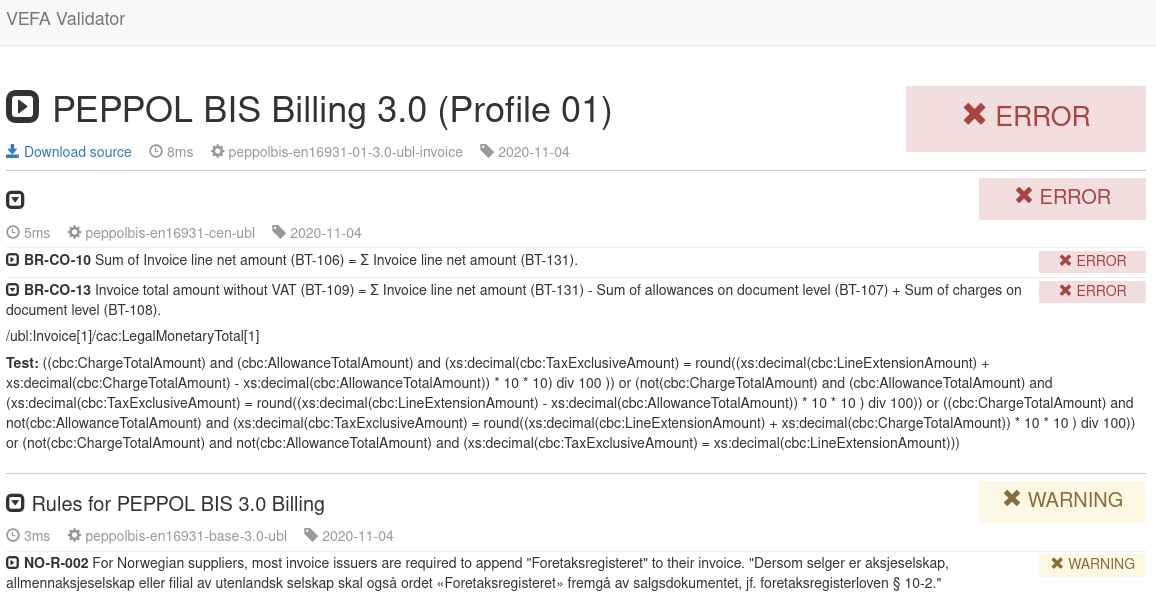
\includegraphics[scale=0.5]{ehfv_validation.png}}
    \caption{\texttt{EHFv3} formāta tiešsaistes validatora rezultāts nevalīdam failam}
    \label{orig:ehf}
\end{figure}
\par Šajā procesā izaicinājumi, ar ko saskārās darba autore, ir pārlieku daudz dati vienam rēķinam un izejošā faila validācija. Izstrādājot datu kartēšanu, labā prakse ir saglabāt tikai nepieciešamo informāciju, kas tiks izmantota turpmākā datu apstrādē. Klienta iesūtītajā \texttt{XML} failā esošais datu formāts saturēja detalizētu informāciju par rēķina precēm, kas nav nepieciešama izvēlētajā izejošajā failā, kas atbilst \texttt{EHFv3} formātam. Šajā gadījumā nepieciešams saprast, kura informācija ir obligāta izejošajam failam. Tieši šim formātam šo šķērsli var pārvarēt, pārlasot formāta dokumentāciju\footnote{https://docs.peppol.eu/poacc/billing/3.0/syntax/ubl-invoice/tree/}. Taču var sanākt situācijas, kad ievaddatos esošie tagi vai to vērtības ir mulsinošas, kas var novest līdz nepareizās informācijas saglabāšanas. Tad nepieciešams sazināties ar klientu un uzzināt atbildes par neskaidrībām.
\par Klienta formātam ir atsevišķi pieejami \texttt{PDF} faili ar nepieciešamajiem datiem, kas būs izmantoti kā pielikumi izsūtītajiem rēķiniem elektroniskajās vietnēs, vai izsūtīti fiziskai saņemšanai pastkastē. \texttt{PDF} failā jau ir ievietota gala saņēmēja adrese dokumenta pirmajā lapā, taču nav ievēroti noteiktie vēstules adreses atrašanās noteikumi, kas redzami \ref{orig:margins} attēlā. Norobežojumi ir noteikti, lai vēstules aploksnes adreses lodziņā nebūtu redzama nekāda papildus informācija par rēķinu. Lai novērstu šo problēmu, tiek pievienota atsevišķa lapa esošajam \texttt{PDF} dokumentam ar ielasīto saņēmēja adresi.
\begin{figure}[H]
    \centering
    \fbox{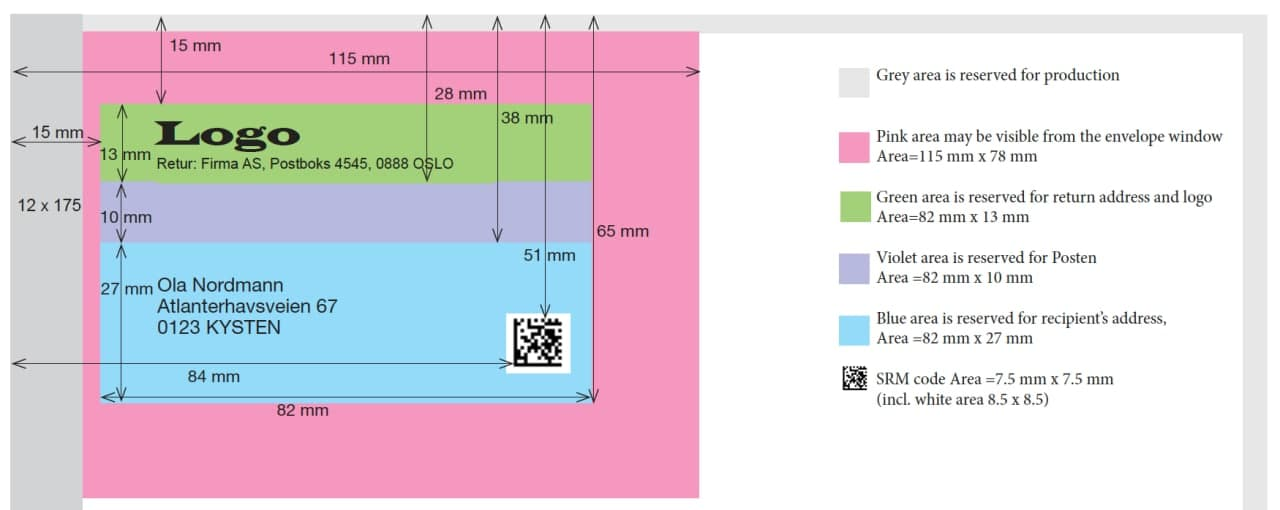
\includegraphics[scale=0.4]{letter-margins.jpg}}
    \caption{Noteiktais saņēmēja adreses un kompānijas logo novietojums vēstulē}
    \label{orig:margins}
\end{figure}
\par Formātā tika izstrādāta papildu kondīcija rēķina saņēmēja adreses saglabāšanai. Adresei uz vēstules jābūt norādītai noteiktā secībā - saņēmēja vārds, ielas nosaukums, pilsēta, pasta kods, valsts -, kas tiek panākts, izmantojot jau esošu skriptu pareizai adreses uzstādīšanai ģenerētajam \texttt{PDF} failam no saņēmēja klases mainīgajiem. Ievadfailos esošās adreses līnijas atsevišķos gadījumos papildu tagā saturēja papildinformāciju, kurai nav izveidots atsevišķs mainīgais saņēmēja klasē un kas izraisīja nepieciešamību pielietot algoritmu, kurā datu vērtības tiktu kondicionāli saglabātas mainīgajos, saglabājot nepieciešamo adreses attēlošanas secību un neizraisot pārlieku garas adreses rindiņas vēstulē.

\subsubsection{ubw}
\par Prakses laikā tika atjaunota maršrutēšanas kvīts. Tas ir atsevišķi ģenerēts fails, kas uzrāda informāciju uzņēmuma klientam par izsūtīto dokumentu piegādes statusu. Pievienojot pie maršrutēšanas kanāliem kvīts ģenerēšanu, klients saņem apkopotus datus par dokumentu piegādes kanālu (mobilās maksāšanas aplikācija, kāds no e-pasta servisiem, dokumentu printēšana, u.c.), piegādes statusu, iespējamo kļūdu dokumenta datos. Maršrutēšanas kvīts var būt izstrādāta pēc uzņēmuma klienta uzskatiem, ievērojot vēlamo datu uzskaiti, datu vizuālo noformējumu vai ģenerētā faila formātu, kas tiek apstrādāts klienta sistēmā.
\par Produkcijā esošā \texttt{xml} faila formāta maršrutēšanas kvīts sastāv no faila galvenes, kas uztur informāciju par failu partijas izveidi, identifikatoru, izmantotajiem maršrutēšanas kanāliem un ielasītā faila nosaukumu, un faila pamatdaļas, kurā ir informācija par ielasītajiem rēķiniem un to piegādes statusiem. Kvīts ģenerēšanas kodā tika pievienots papildus veids faila nosaukuma iegūšanai iepriekšējās metodes neveiksmīga rezultāta dēļ, un ir pievienota pārbaude priekš datu piegādes statusa noteikšanas. Papildinātais kods tika pārbaudīts pie vairākiem ienākošo failu veidu gadījumiem - ar valīdiem datiem, ar vairāku rēķinu un viena rēķina datiem viena failā, ar nevalīdiem failiem (piem., rēķina detaļu cenu summa, ieskaitot pievienotos nodokļus un atlaides, nesakrīt ar kopējo rēķina summu) un ar failiem, kas izsauktu ienākošo failu partijas (angl. batch) kļūdu failu apstrādē. Testēšana iekļāva arī dažādu failu ielasīšanas konfigurāciju maršrutēšanas kanāliem, kur var pielietot ienākošās failu partijas ielasīšanu kā vienu kopumu vai katru failu atsevišķi, iespēja noteikt vai par katru ielasīto failu tiks ģenerētas atsevišķas kvītis vai vienā kvītī būs apkopota informācija par visiem ielasītajiem failiem.


\subsubsection{templates}
\par Prakses laikā tika atjauninātas vairākas datu veidnes. Veidņu atjaunināšana parasti iekļauj statiskā jeb nemainīgā teksta ievietošanu vai atjaunināšanu veidnē, noteiktu vizuālo elementu kā, piemēram, attēlu, tabulu, formatējuma izņemšanu vai pievienošanu veidnē. Izmaiņas tiek testētas ar atbilstošajiem ienākošajiem failiem, kas ietekmē veidnes izkārtojumu. Pēc veiksmīgas pārbaudes, izveidotie faili tiek nosūtīti klientam uz apstiprināšanu. Apstiprinātās izmaiņas tiek pievienotas jau produkcijā esošajā kodā.
% \par

\subsubsection{e-pasta template}
\par Tika izstrādāta jauna e-pasta veidne, kas lielākoties iekļauj statisko tekstu. Mainīgais teksts tiek ievietots e-pasta tematā un sūtītāja e-pasta adresē, atsevišķos gadījumos arī galvenajā tekstā. E-pasta veidne tiek veidota, ievērojot \texttt{html} koda struktūru un sintaksi. E-pastā iekļautais teksts un tā izkārtojums var būt pārbaudīti, ievietojot veidnes saturu tiešsaistes \texttt{html} koda rezultāta skatītājos (angl. viewer) vai nosūtot e-pastu caur uzņēmuma testēšanas mājaslapu koda testētājam.
\subsubsection{prasmju pielietojums}
\par Pietiekama darba izpildei kompānijā ir nepieciešamas pamata zināšanas programmēšanā, pārējās pramses bija iemācītas darba laikā. No augstskolā apgūtajām zināšanām darba autore prakses laikā pielietoja programmēšanas pamatzināšanas, \texttt{Java} programmēšanas valodas zināšanas. Dažādos gadījumos, kur bija nepieciešams izstrādāt kondicionālas pārbaudes un datu apstrādes, nepieciešamas matemātiskās loģikas un būla funkciju izpratnes prasmes. Kritiskā domāšana un prasme strādāt komandā ir noderīgas priekš veiksmīgas un ātras projekta izstrādes. \texttt{Git} versijas kontroles zināšanas un izmantošana ir nepieciešamas prasmes projektu veikšanā, lai sekotu līdzi koda izmaiņām.



% \par
% Uzņēmuma vai organizācijas apraksts; uzņēmuma vai organizācijas organizatoriskā  struktūra; pārskats par prakses gaitu; profesionālās darbības pamatuzdevumu veikšanai nepieciešamo prasmju pieliet